\chapter{Programming tools for robotics}\label{ch:hatchery}
\setlength{\epigraphwidth}{0.78\textwidth}
\epigraph{``The hope is that, in not too many years, human brains and computing machines will be coupled together very tightly, and that the resulting partnership will think as no human brain has ever thought and process data in a way not approached by the information-handling machines we know today.''}{\begin{flushright}--Joseph \citet{licklider1960man}, \href{https://groups.csail.mit.edu/medg/people/psz/Licklider.html}{\textit{Man-Computer Symbiosis}}\end{flushright}}

In this chapter we will discuss the design and implementation of an integrated development environment (IDE) for building intelligent robotic software. Modern robots are increasingly driven by systems which learn and improve over time. Most researchers would agree that modern robotic systems have not yet achieved biologically competitive sensorimotor capabilities and most intelligent systems are not physically embodied. However, it is our view that any closed-loop control system that is not explicitly programmed to perform a specific task, but which learns it from experience is an \textit{intelligent system}. Furthermore, any closed-loop system with physical motors is a \textit{robotic system}. While research has demonstrated successful applications in both areas separately, it is widely believed the integration of intelligent systems and robotics will be tremendously fruitful when fully realized.

Hatchery is a tool designed to assist programmers writing robotics applications using the ROS middleware. At the time of its release, \href{https://github.com/duckietown/hatchery}{Hatchery} was the first ROS plugin for the \href{https://www.jetbrains.org/intellij/sdk/docs}{IntelliJ Platform} \footnote{An IDE platform for C/C++, Python and Android development, among other languages.}, and today, is the most widely used with over 10,000 unique downloads. While the idea is simple, its prior absence and subsequent adoption suggest there is unmet demand for such tools in the development of intelligent software systems, particularly in domain-specific applications like robotics.
%

\begin{figure}
    \centering
    \begin{tikzpicture}
        \begin{axis}[
            ybar, ymin=0,
            ylabel=Downloads,
            date coordinates in=x,
            xmin=2017-12-01,
            xmax=2019-06-01,
            xtick=data,
            xticklabel style={
                rotate=70,
                anchor=near xticklabel,
            },
            xticklabel=\year-\month,
            nodes near coords,
            nodes near coords align={vertical},
            height=0.25\textwidth,
            width=0.95\textwidth,
            enlarge x limits=0.03,
            axis x line*=bottom,
            axis y line*=left,
            tick pos=left,
            compat=newest,
        ]
            \addplot table[col sep=comma, x=Category,y=Downloads]{../data/hatchery_downloads.csv};
        \end{axis}
        \node[above,font=\large\bfseries] at (current bounding box.north) {Unique downloads of Hatchery};
    \end{tikzpicture}
    \caption{Unique downloads of Hatchery between the time of its release and June 2019. \url{https://plugins.jetbrains.com/plugin/10290-hatchery}.}
    \label{fig:hatchery_downloads}
\end{figure}
%
\section{Introduction to the Robot Operating System}

The \href{https://www.ros.org/}{Robot Operating System} (ROS)~\citep{quigley2009ros} is a popular middleware for robotics applications. At its core, ROS provides software infrastructure for distributed messaging, but also includes a set of community-developed libraries and graphical tools for building robotics applications. ROS is not an operating system (OS) in the traditional sense, but it does support similar functionality such as shared memory and inter-process communication. Unlike pure message-oriented systems such as DDS~\citep{pardo2003omg} and \href{https://zeromq.org/}{ZMQ}~\citep{hintjens2013zeromq}, in addition to the communication infrastructure, ROS provides specific APIs for building decentralized robotic systems, particularly those which are capable of mobility. This includes standard libraries for serializing and deserializing geometric data, coordinate frames, maps, sensor messages, and imagery.

The ROS middleware provides several language front-ends for polyglot programming. According to one community census taken in 2018, 55\% of all ROS applications on GitHub are written in C/C++, followed by Python with a 25\%~\citep{Areserio54:online} developer share. Source code for a typical ROS application contains a mixture of C/C++ and Python code, corresponding to the respective language preferences in the robotics and machine learning communities. Hatchery is compatible with most common ROS client libraries, including \href{https://wiki.ros.org/rosjava}{rosjava} for Java, \href{https://wiki.ros.org/rospy}{rospy} for Python, \href{https://wiki.ros.org/rospy}{roscpp} for C/C++, and other language front ends.

\begin{figure}
    \centering
    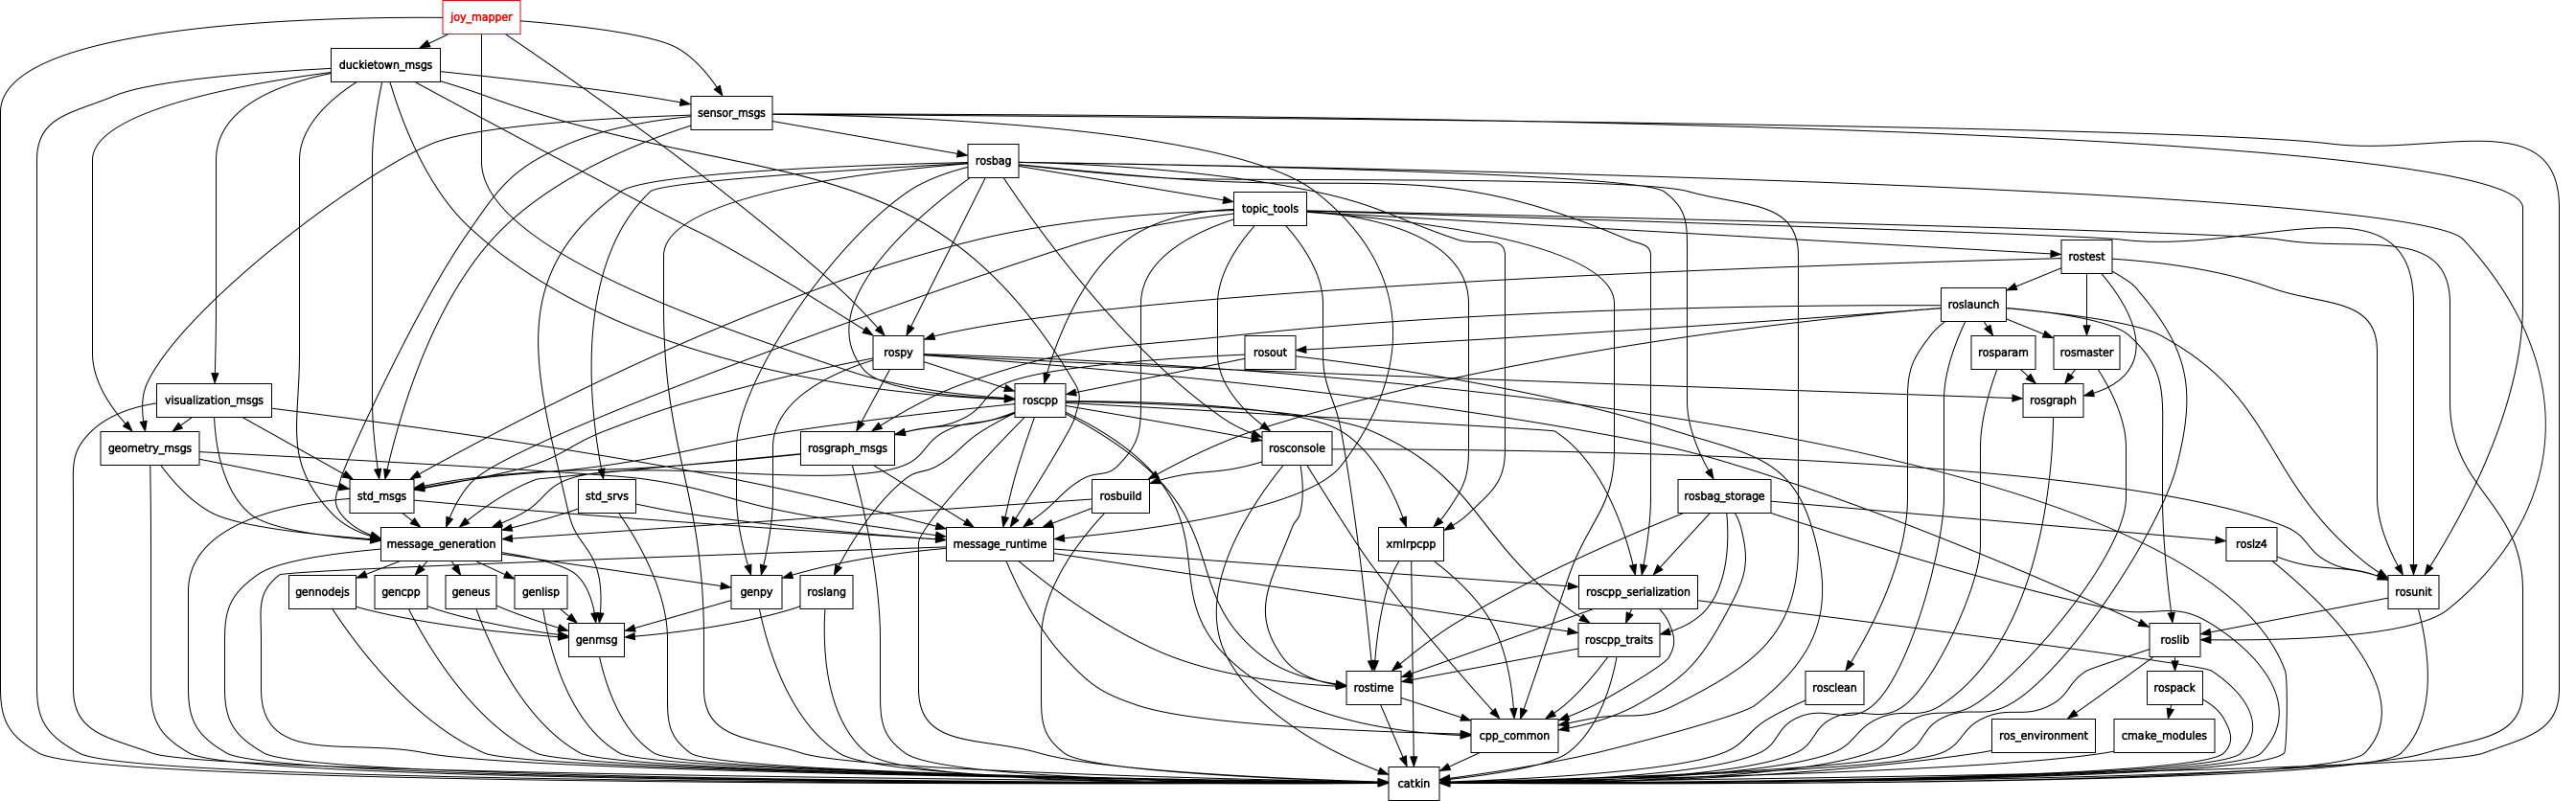
\includegraphics[width=\textwidth]{../figures/rqt_dep_graph.png}
    \caption{A typical ROS application contains a large graph of dependencies.}
\end{figure}

A typical ROS project has several components, including the source code, configuration files, build infrastructure, compiled artifacts and the deployment environment. To build a simple ROS application, several steps are necessary. First, one must install the ROS system, which is only officially supported on Debian-based Linux distributions.\hspace{-.08em}\footnote{Detailed installation instructions may be found here: \url{https://wiki.ros.org/ROS/Installation}}
%
Assuming ROS has been installed to the default location, it can be sourced like so:
%
\begin{pclisting}
    ~$ source /opt/ros/<ROS DISTRO>/setup.[ba]sh
\end{pclisting}
%
A minimal ROS application contains at least one \textit{publisher} and \textit{subscriber}, which pass messages over a shared communication channel. The publisher might be defined as follows:
%
\begin{pythonlisting}[title=./catkin\_ws/src/pubsub/publisher.py]
import rospy
from std_msgs.msg import String

pub = rospy.Publisher("(*@\hl{channel}@*)", String, queue_size=10)
rospy.init_node("publisher", anonymous=True)
rate = rospy.Rate(10)
while not rospy.is_shutdown():
pub.publish("Some message")
rate.sleep()
\end{pythonlisting}
%
As the publisher writes messages to \hl{\ttfamily\small channel}, another node which is subscribed to the same channel will receive a callback when new messages arrive and can read them off the channel:
%
\begin{pythonlisting}[title=./catkin\_ws/src/pubsub/subscriber.py]
def callback(data):
    rospy.loginfo(rospy.get_caller_id() + "received data %s", data.data)

    rospy.init_node("subscriber", anonymous=True)
    rospy.Subscriber("(*@\hl{channel}@*)", String, callback)
    rospy.spin()
\end{pythonlisting}
%
All ROS packages have launch file, which contain a manifest of available nodes:
%
\begin{launchlisting}[title=./catkin\_ws/src/pubsub/pubsub.launch]
<launch>
<node name="publisher" pkg="pubsub" type="publisher.py" output="screen"/>
<node name="subscriber" pkg="pubsub" type="subscriber.py" output="screen"/>
</launch>
\end{launchlisting}
%
To build and run the application, the following series of commands are required:
%
\begin{pclisting}
    ~$ cd catkin_ws && catkin_make
\end{pclisting}
%
\begin{pclisting}
~$ roslaunch pubsub pubsub.launch
\end{pclisting}
%
Rather than interacting with the command line, it would be convenient to have a graphical tool to perform all of these tasks automatically. Additionally, it would be helpful to detect if there were a typographical error or navigable reference in the launch file:
%
\begin{launchlisting}[title=./catkin\_ws/src/pubsub/pubsub.launch]
<launch>
<node name="publisher" pkg="pubsub" type="(*@\color{red}\textbf{pubsher.py}@*)" output="screen"/>
<node name="subscriber" pkg="pubsub" type="(*@\color{blue}\underline{subscriber.py}@*)" output="screen"/>
</launch>
\end{launchlisting}
%
Notice how the typographical error is printed in red and the valid file reference is underlined in blue, indicating it can be selected to open the file shown above. Broadly, these are the kinds of features IDEs provide and are examples of specific functionality in Hatchery.

\section{Installation}\label{subsec:installation}

\noindent To simply run the tool, users should have the following software dependencies:
%
\begin{enumerate}
\item MacOS or Debian-based Linux distribution
\item Robot Operating System (Electric Emys or later)
\item Java SE (JRE 8+) or CLion/PyCharm 2019.1+
\end{enumerate}
%
\noindent ROS users can use the following command to open an existing ROS project:
%
\begin{pclisting}
~$ git clone https://github.com/duckietown/hatchery && cd hatchery && \
   ./gradlew runIde [-Project="<ABSOLUTE_PATH_TO_ROS_PROJECT>"]
\end{pclisting}
%
\noindent Duckietown users can simply use \inline{dts}, the Duckietown Shell:
%
\begin{dtslisting}
dt> hatchery
\end{dtslisting}
%
\noindent Hatchery can also be installed directly from inside the CLion or PyCharm IDEs, via the following menu options: \menu{File > Settings > Plugins > Marketplace > {\faSearch ``Hatchery''}}

\section{Plugin development}

To build an IDE, some tools are helpful. First, is an IDE, and its source code. Assume that IDE\textsubscript{0} exists. In order to build a new IDE, IDE\textsubscript{1}, we can load the source code from IDE\textsubscript{0} into IDE\textsubscript{0} and use IDE\textsubscript{0}, to modify, compile and re-run the code, which becomes IDE\textsubscript{1}, in which the process is repeated. However, this approach has some disadvantages. First, most IDEs are already quite cumbersome to compile and run. As most auxiliary features are small by comparison, modern IDEs have adopted a modular design, which allows them to load specific packages (i.e.\ \textit{plugins}) as needed. So most developers can skip the first step, and load their plugin inside IDE\textsubscript{0} directly. It is still convenient to have the platform source code for reference purposes, but in most cases this code is read-only.

Hatchery uses the \href{https://www.jetbrains.org/intellij/sdk/docs/}{IntelliJ Platform}, an IDE platform which supports most common programming languages. By targeting a platform with support for polyglot programming, we are able to focus on language-agnostic features in the ROS ecosystem, such as parsing and editing ROS-specific configuration files, build and run configuration and other common development tasks.

\subsection{Refactoring}\label{subsec:refactoring}

Refactoring is an essential feature in any IDE, and the essence of refactoring is renaming. Consider what must occur when a user wishes to rename a token in her program, such as the parameter named \inline{data} on line \#1 below:
%
\begin{pythonlisting}
def callback(data):
    rospy.loginfo(rospy.get_caller_id() + "received data: %s", data.data)
\end{pythonlisting}
%
If she were using the \inline{vim} text editor, one solution would be to replace all textual occurrences of the string \inline{data} within the file using \inline{:\%s/data/msg/g}, producing the following result:
%
\begin{pythonlisting}
def callback((*@\hl{msg}@*)):
    rospy.loginfo(rospy.get_caller_id() + "received (*@\hl{msg}@*): %s", (*@\hl{msg}@*).(*@\hl{msg}@*))
\end{pythonlisting}
%
There were four occurrences of the string \inline{data}, only two of which were correctly renamed. Instead, only those strings which refer to the function parameter should be renamed:
%
\newcommand{\cfbox}[2]{\colorlet{currentcolor}{.}{\color{#1}\fbox{\color{currentcolor}#2}}}

\begin{pythonlisting}
def callback((*@\cfbox{red}{data}@*)):
    rospy.loginfo(rospy.get_caller_id() + "received data: %s", (*@\cfbox{red}{data}@*).data)
\end{pythonlisting}
%
Generally, we would like the ability to rename identifiers across files and languages. To do so, we need a richer understanding of code that transcends text -- we need a parser.

\subsection{Parsing}\label{subsec:the-parser}

One of the most important and unappreciated components of an IDE is the parser. Unlike compilers, most IDEs do not use recursive descent or shift-reduce parsing as treated in most compiler textbooks~\citep{appel2003modern}, as these algorithms are not well-suited for real-time editing of source code. Edits are typically short, localized changes inside a large file, and are frequently invalid or incomplete between keystrokes. As most IDEs are expected to recover from local errors and provide responsive feedback while editing source code, re-parsing the entire program between minor edits would be expensive and unnecessary. In order to analyze source code undergoing simultaneous modification and provide interactive feedback, special consideration must be taken to ensure robust and responsive parsing.

Various techniques have been developed to improve the responsiveness of modern parsers. Incremental parsing techniques like those first proposed in \citet{ghezzi1979incremental} and further developed by \citet{wagner1997practical,wagner1997incremental} seek to incorporate caching and differential parsing to accelerate the analysis of programs under simultaneous modification. Fuzzy parsing techniques like those described in ~\citet{koppler1997systematic} aim to increase the flexibility and robustness of parsing in the presence of local errors. Both of these techniques have played a role in the development of language-aware programming tools, which must be able to provide rapid and specific feedback whilst the user is typing.

The procedural instructions for modern parsers are seldom written by hand unless the language being parsed is very simple or raw performance is desired. Even parsers designed for IDEs, where incremental parsing and error-tolerance is so important, metacompilation toolkits such as ANTLR~\citep{parr1995antlr}, or Xtext~\citep{eysholdt2010xtext} cover a surprising number of common use-cases. Hatchery uses \href{https://github.com/JetBrains/grammar-kit}{Grammar-Kit}, a toolkit designed to assist users developing custom language plugins for the \href{https://www.jetbrains.org/intellij/sdk/docs}{IntelliJ Platform}. It uses a DFA-based lexer generator, JFlex~\citep{klein2001jflex}, and a custom parser-generator loosely based on the parsing expression grammar (PEG)~\citep{ford2004parsing}, a descendant of the Backus-Naur Form (BNF) grammar specification. This specification is consumed by the GrammarKit parser generator and translated to Java source code, producing a parser which reads source code written in the specified language and constructs a program structure interface (PSI), the IntelliJ Platform's internal data structure for representing abstract syntax trees (ASTs). Here is an excerpt of a PEG BNF grammar for parsing ROS \href{https://wiki.ros.org/msg}{\inline{.msg}} files:
%
\begin{bnflisting}
rosInterfaceFile ::= ( property | COMMENT )*
property ::= ( TYPE FIELD SEPARATOR CONSTANT ) | ( TYPE FIELD ) {
    pin=3 // Identifies an unambiguous delimiter or fallback point
    recoverWhile="recover_property" // Error recovery predicate
    mixin="edu.umontreal.hatchery.psi.impl.RosMsgNamedElementImpl"
    implements="edu.umontreal.hatchery.psi.RosMsgNamedElement"
    methods=[getType getKey getValue getName setName getNameIdentifier]
}
private recover_property ::= ! ( TYPE | FIELD | SEPARATOR | COMMENT )
\end{bnflisting}
%
\begin{figure}
\centering
% To regenerate: https://homepage.ruhr-uni-bochum.de/jan.holthuis/posts/using-the-latex-rail-package#manual-compilation-and-latexmk-support
\begin{rail}
( [2] TYPE FIELD ( () | SEPARATOR CONSTANT) ) | ( [1] COMMENT )
\end{rail}
\caption{Railroad diagram for the grammar shown above (reads from left to right).}
\label{fig:railroad}
\end{figure}
%
The lexical rules for the tokens, \inline{TYPE}, \inline{FIELD}, \inline{CONSTANT} et al. are defined in a separate \inline{.flex} file, the \href{https://www.jflex.de/manual.html#Grammar}{JFlex grammar}. Below is an excerpt from the accompanying \inline{.flex} lexer:
%
\begin{flexlisting}
TYPE_CHARACTER=[^:=#\ \r\n\t\f\\]
FIELD_CHARACTER=[^:=#\ \r\n\t\f\\]
SEPARATOR_CHARACTER=[:=]
CONSTANT_CHARACTER=[^\r\n\f#]
COMMENT_CHARACTER=#[^\r\n\f]*
\end{flexlisting}

Grammar-Kit consumes these files and generates Java source code for parsing ROS \href{https://wiki.ros.org/msg}{\inline{.msg}} files. Generated sources can be manually refined to provide support for more advanced functionality such as more flexible error-recovery. For regular languages like the interface description languages (IDL) found in ROS \href{https://wiki.ros.org/msg}{\inline{.msg}} and \href{https://wiki.ros.org/srv}{\inline{.srv}} files, the default generated parser and lexer are usually sufficient. Hatchery is also capable of parsing \href{https://wiki.ros.org/urdf}{URDF}, \href{https://wiki.ros.org/Manifest}{package manifest} and \href{https://wiki.ros.org/roslaunch/XML}{roslaunch} XML.

\subsection{Running and debugging}

The process of compiling and running ROS applications often requires several steps, ex.:
%
\begin{pclisting}
~$ . /opt/ros/<DISTRO>/setup.[ba]sh &&
   cd <PROJECT>/catkin_ws &&
   catkin_make &&
   . devel/setup.sh &&
   [export ROS_MASTER_URI=<URI> &&]
   roslaunch [OPTIONS] src/.../<LAUNCH FILE> [ARGUMENTS]"
\end{pclisting}
%
Hatchery provides assistance for configuring, building and running ROS applications inside a custom graphical user interface (GUI). This GUI effectively serves as a wrapper for the ROS command line interface (CLI). Visual elements like configuration options and command line flags are written to an internal model called the ``Run Configuration'' (\autoref{fig:ros_run_config}). When a run configuration is manually triggered, Hatchery's internal model is serialized to a \inline{String}, representing the command to be executed. This \inline{String} is then sent to a terminal emulator, which invokes the command and displays the corresponding output.

\begin{figure}
\centering
\frame{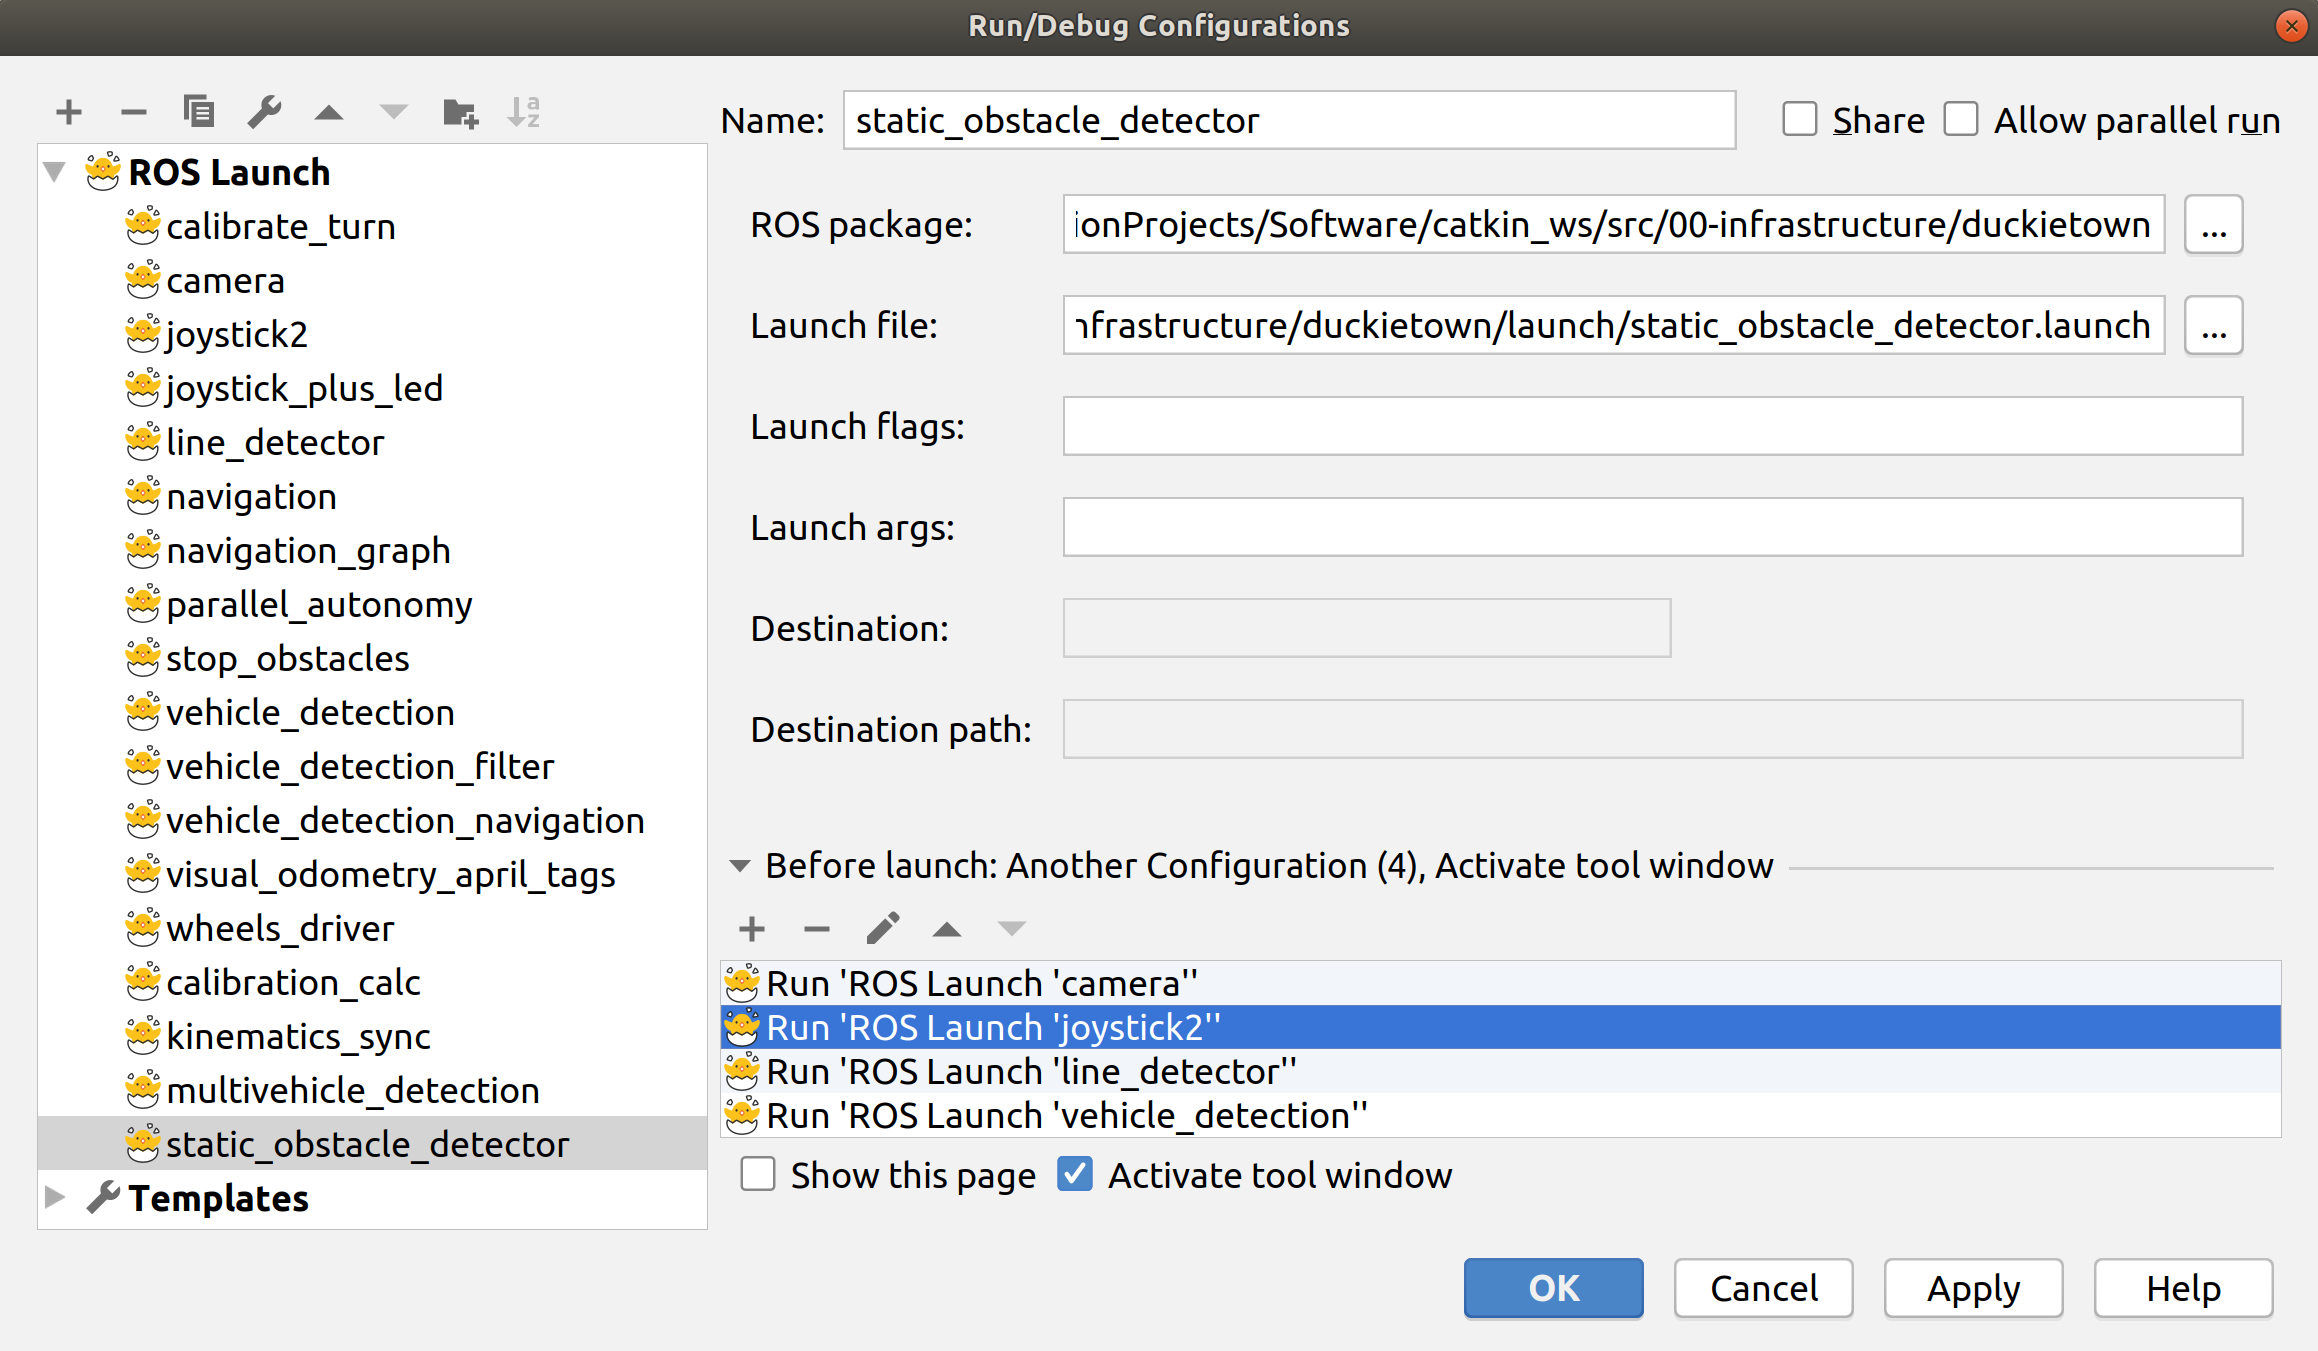
\includegraphics[width=0.90\textwidth]{../figures/ros_run_config.png}}
\caption{ROS Run Configuration. Accessible via: \menu{Run > Edit Configurations > + > ROS Launch}}
\label{fig:ros_run_config}
\end{figure}

\subsection{User interface}

An often overlooked, but important aspect of development tools is the graphical user interface, as the primary interface for editing source code. In the early days of modern computing, the only way of getting information in or out of a computer involved punching holes in paper. Later, computers were equipped with technology to emit the same binary pattern as pixels, which could be used to display a small alphabet called ASCII. With higher density and frequency displays, computers could render more sophisticated shapes and animations. These improvements are the direct result of graphical innovation, but can also be seen as progress in program representation, where the symbolic medium was itself just a notational convention which developers and machines used to communicate.

\begin{figure}
\centering
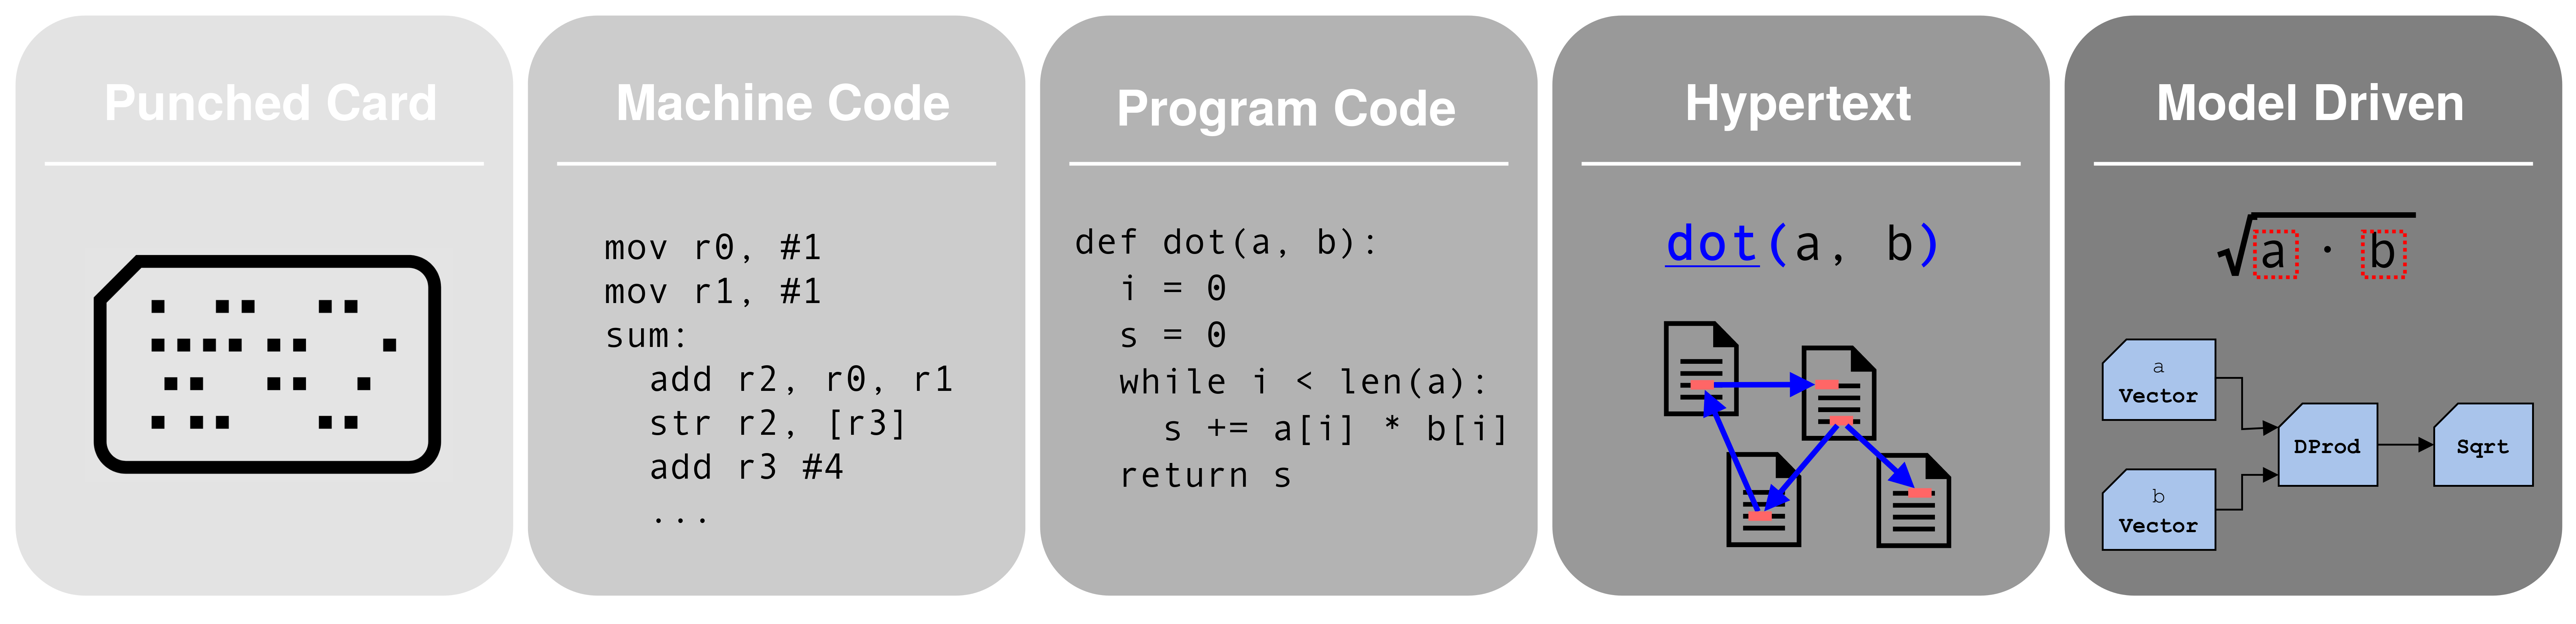
\includegraphics[width=0.90\textwidth]{../figures/progress_in_program.png}
\caption{The evolution of code. On the left are languages that force the user to adapt to the machine. To the right are increasingly flexible representations of source code.}
\label{fig:evolution_of_programming}
\end{figure}

ASCII is still the dominant medium for modern programming, although machines still use various forms of low-level assembly code for execution. A great deal of software infrastructure is dedicated to translating between such representations via programming languages and compilers. While many software frameworks provide a minimal command line interface (CLI) and some even provide sophisticated programming environments, these tools are fairly restrictive. In the same way that early computer scientists probably did not invent new algorithms by imagining patterns of holes in paper, ASCII is also an indirect medium for expressing ideas, albeit one slightly less contrived. As hardware and software technology progressed, programming languages moved ``up the stack'', allowing their users to express ideas in a notation which was more familiar and easy to reason about its execution.

\begin{figure}
\centering
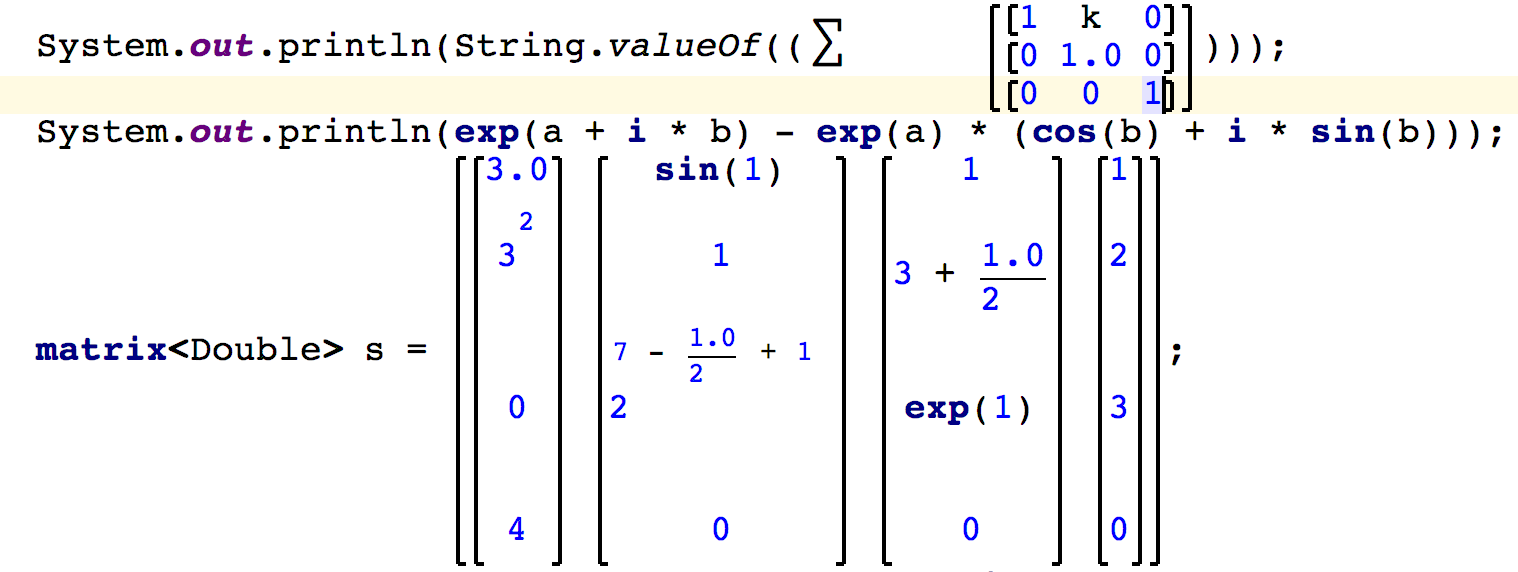
\includegraphics[width=0.90\textwidth]{../figures/mps_screenshot.png}
\caption{Projectional editors such as \href{https://www.jetbrains.com/mps/}{MPS}~\citep{voelter2010language, pech2013jetbrains} (shown above) are able to render source code in visually creative ways. This might resemble freehand notation or some other visually appealing format.}
\label{fig:mps_screenshot}
\end{figure}

With the development of modern languages came programming tools capable of representing code as a mixture of hypertext and graphical user interfaces. Such tools provide a richer representation for code than plaintext and help to capture programs' graph-based structure, but still use ASCII with sparse visual cues to render code. Some tools support larger character sets and font-based typographic ligatures, although the visual representation of source code remains mostly linear and textual.

More experimental UIs, as proposed in the language oriented programming~\citep{dmitriev2004language} and model-driven engineering~\citep{famelis2015mummint} literature, suggest the possibility of more visually flexible layouts. This uncoupling between the composition and representation of text raises many intriguing questions. With the proliferation of new abstractions and programming shorthands, what is the appropriate level of notation required for a given programming task? And who is the intended audience? These are important questions to consider when designing a new programming tool.

The Hatchery plugin provides a lightweight GUI overlaying the program's source code. This interface (\autoref{fig:hatchery_gui}) primarily consists of simple visual cues such as text highlighting, navigation assistance and other menus and configuration panels for performing various programming tasks. The host IDE offers a visual language consisting of iconography and repetitive visual motifs, which serve as cognitive landmarks to guide the developer's procedural memory. The IntelliJ Platform offers a palette of common design elements, which users who are familiar with the IDE can recognize at a glance. Plugins can use these same patterns to access procedural memories implanted in the userbase, facilitating transfer learning. To do this properly requires familiarity with the design language and careful integration with the target framework (i.e. ROS).

Hatchery provides a settings menu for configuring and managing ROS installations which can automatically detect local ROS distributions and also allows users to manually configure the \href{https://wiki.ros.org/ROS/Tutorials/InstallingandConfiguringROSEnvironment}{ROS environment}, as shown in ~\autoref{fig:ros_settings}.
%
\begin{figure}[b]
\centering
\frame{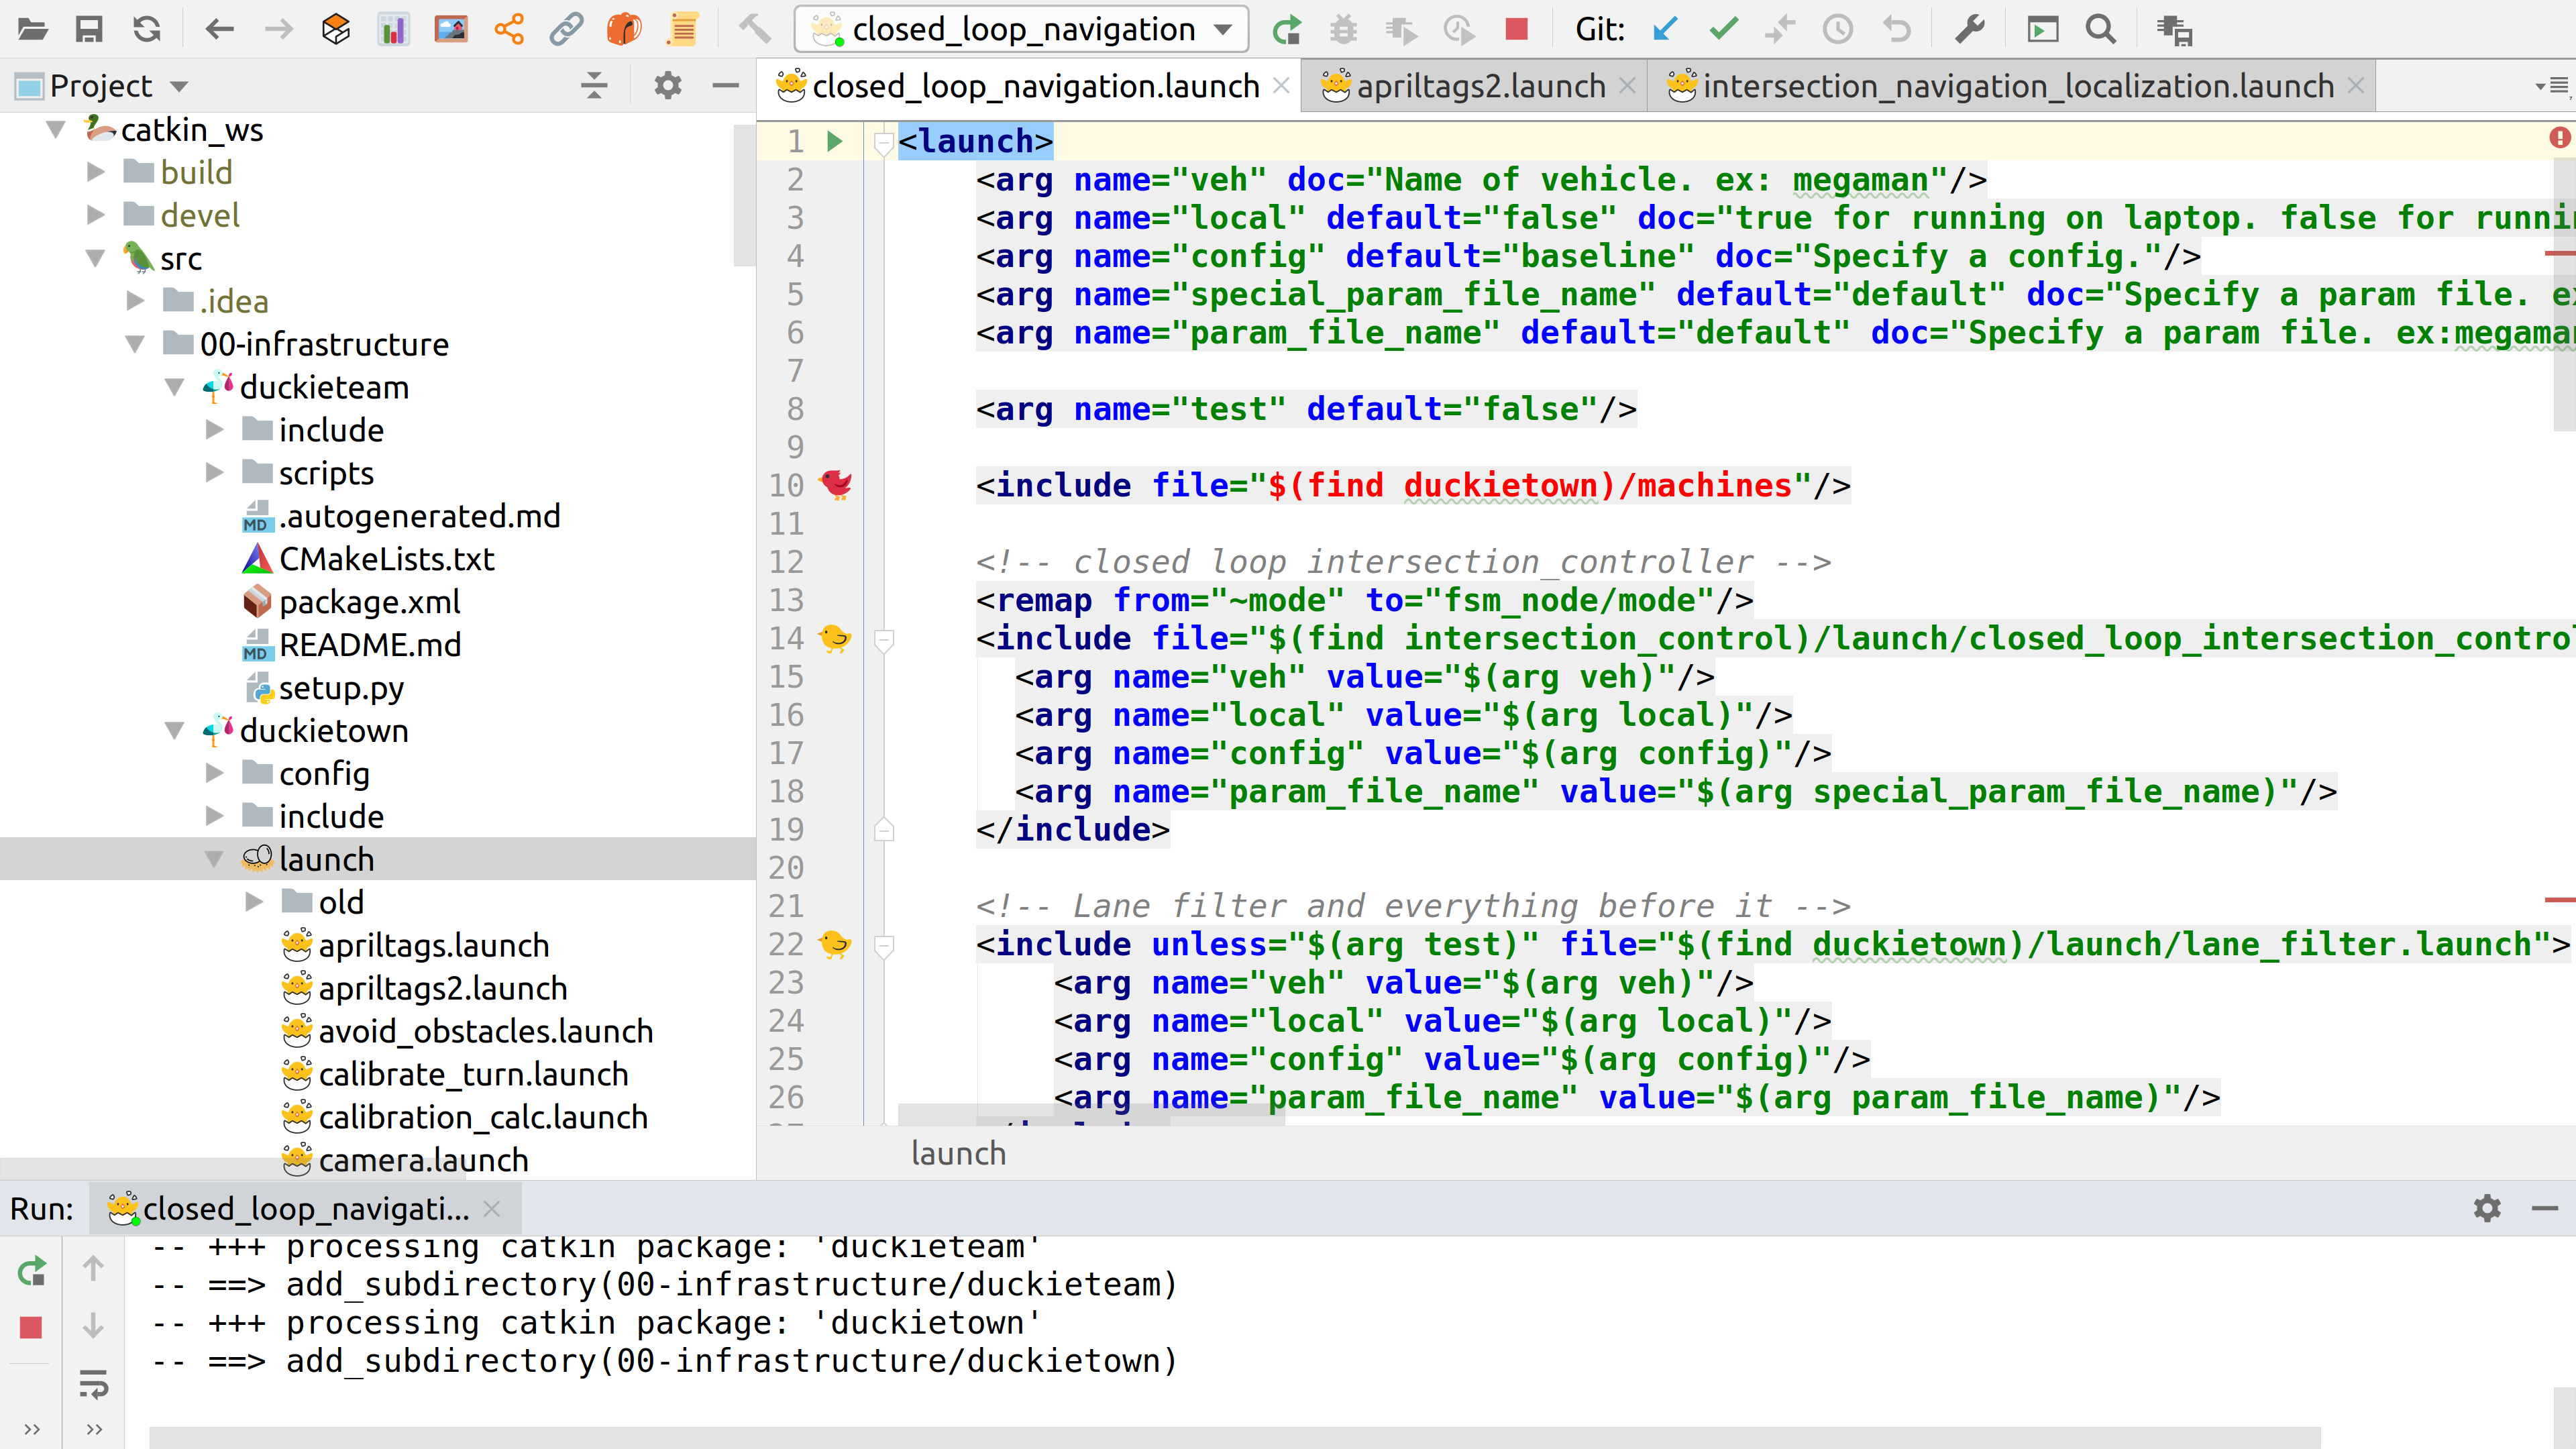
\includegraphics[width=0.90\textwidth]{../figures/hatchery_screenshot.png}}
\caption{Hatchery UI supports syntax highlighting, validation and project navigation.}
\label{fig:hatchery_gui}
\end{figure}
%
\begin{figure}
\centering
\frame{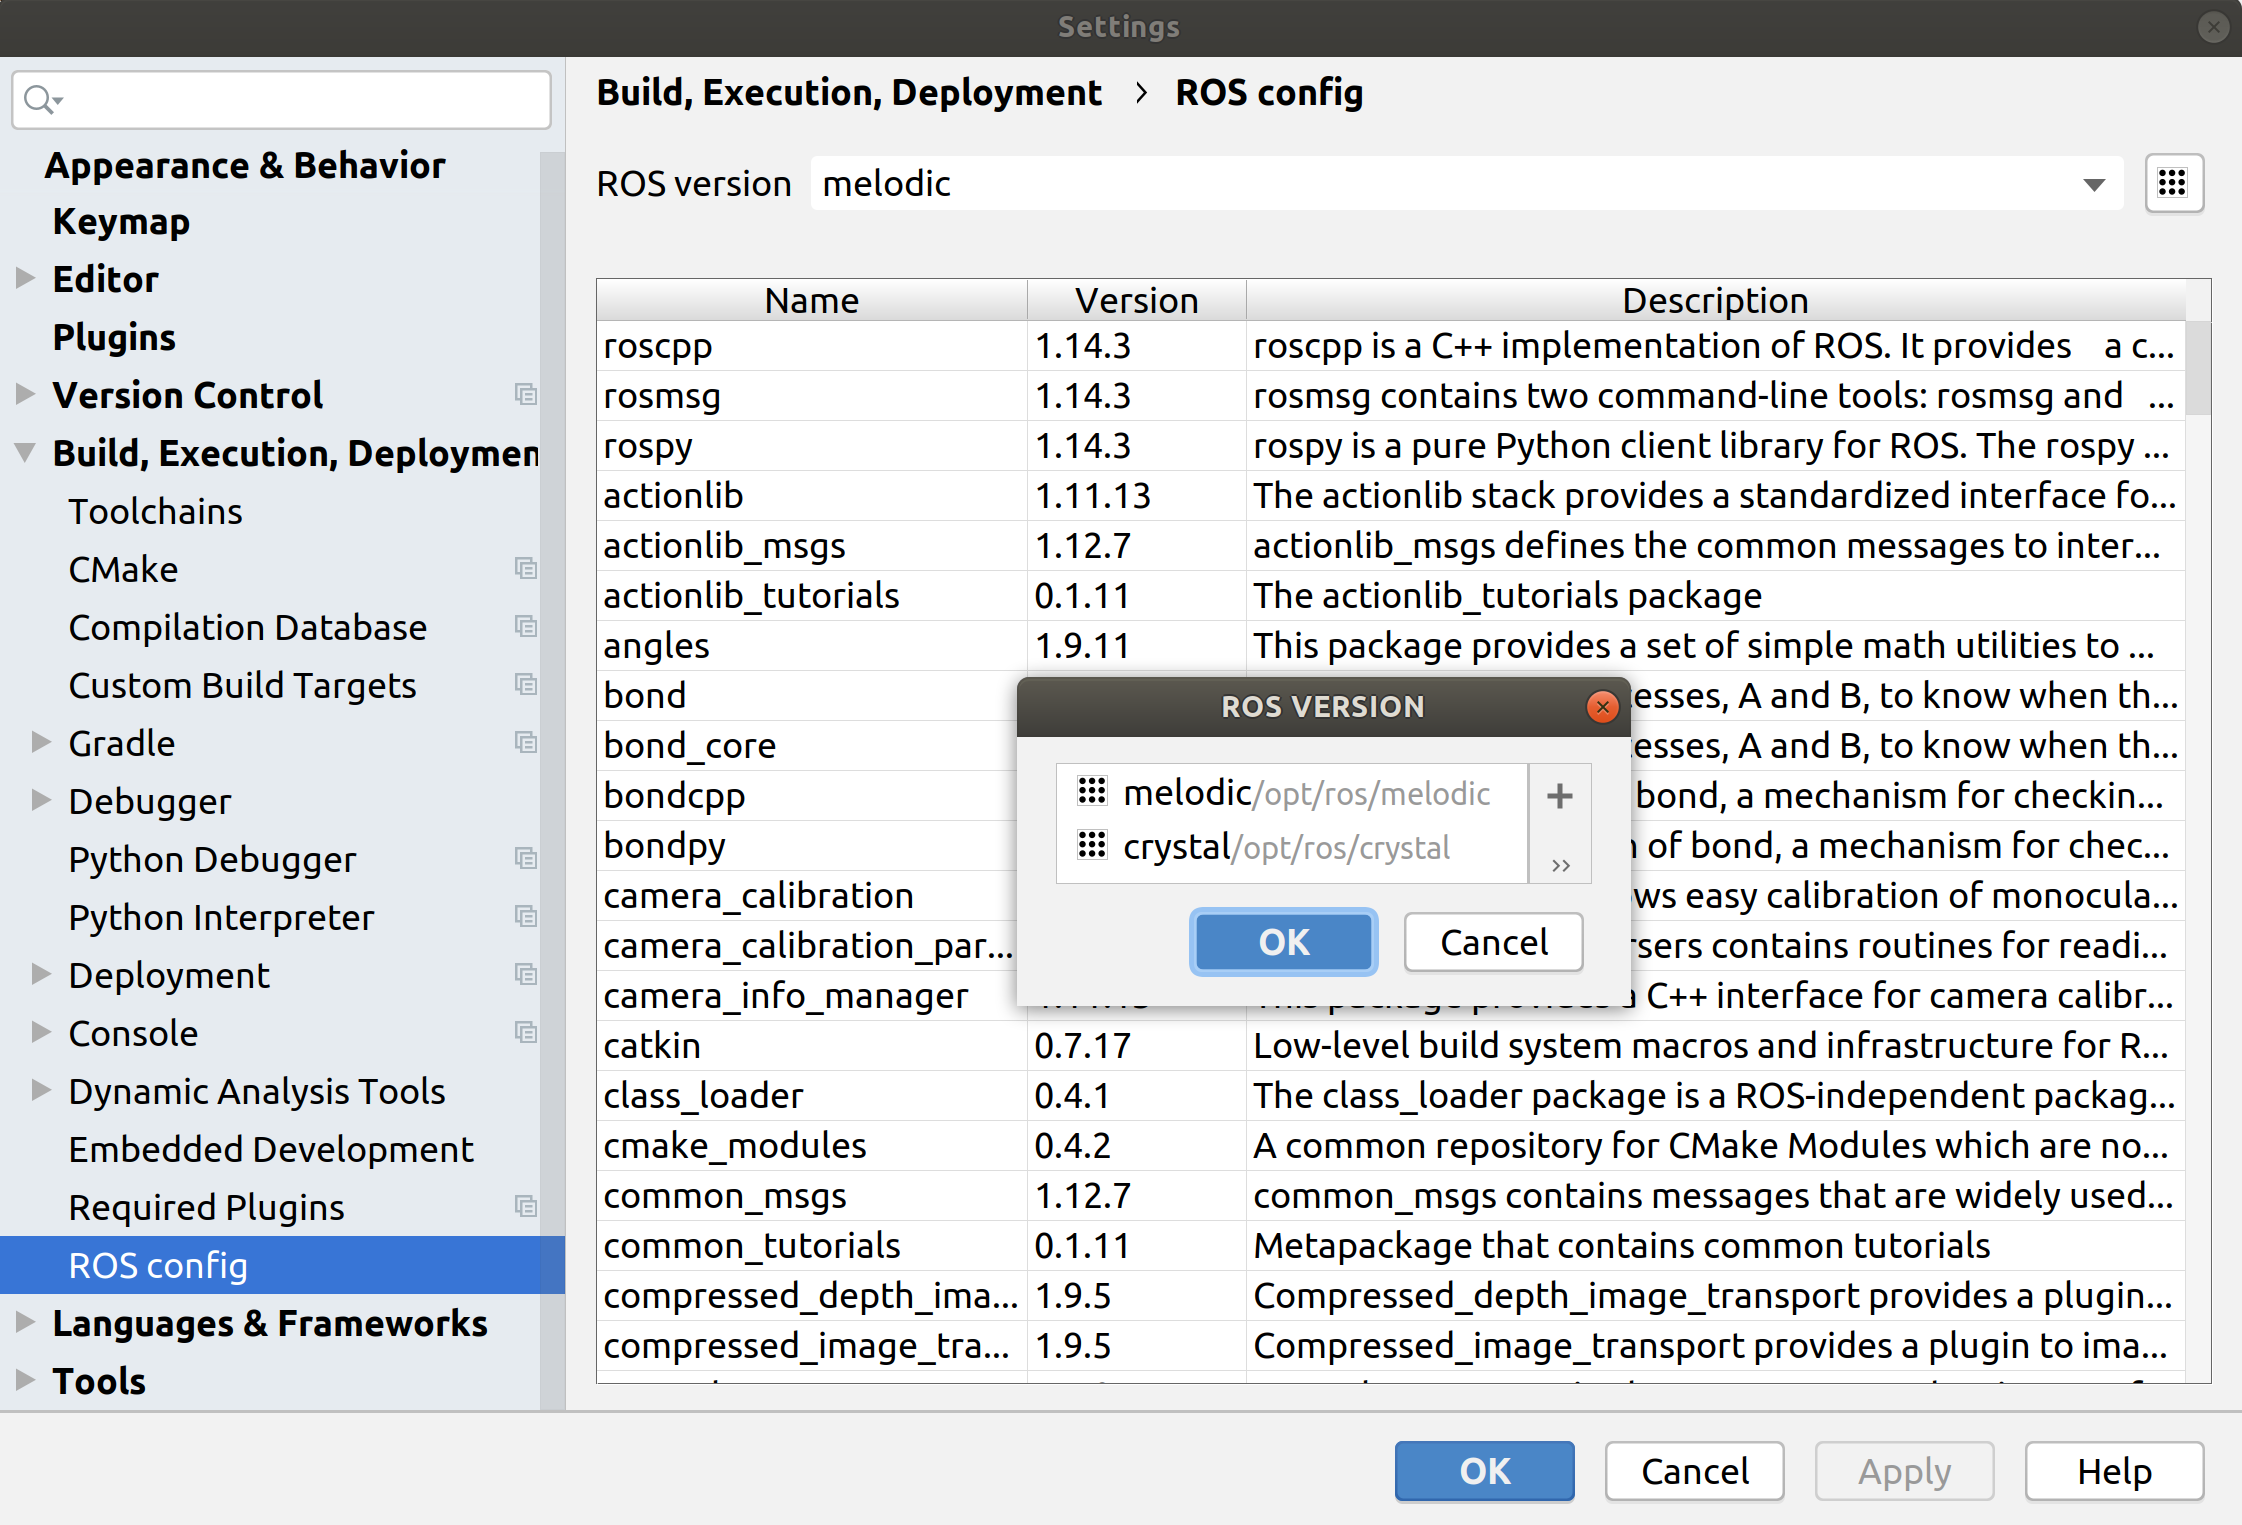
\includegraphics[width=0.90\textwidth]{../figures/ros_settings.png}}
\caption{Detection of local ROS packages. Accessible via: \menu{File > Settings > ROS config}}
\label{fig:ros_settings}
\end{figure}

\section{Ongoing work}

\noindent While it supports many common use cases such as rudimentary code navigation, static analysis and run assistance, Hatchery is currently a work in progress. We are working to expand Hatchery's support for ROS programming in some of the following areas:\vspace{10pt}
%
\begin{itemize}
\item \textbf{Syntax support} -- Highlighting, navigation, autocompletion
\item \textbf{Program analysis} -- Code inspections, intentions, and linting
\item \textbf{Testing support} -- Unit and integration testing, code coverage
\item \textbf{Project creation} -- Project setup and boilerplate code generation
\item \textbf{Dependency management} -- Track installed and missing packages
\item \textbf{Monitoring utils} -- Logging, diagnostics, profiling and visualization
\item \textbf{Crash analytics} -- Enhanced stack traces with source navigation
\item \textbf{Build automation} -- Delta rebuilds, cmake magic, code hotswap
\item \textbf{ROS integration} -- Nodes, topics, services, parameters, graphs
\item \textbf{Duckumentation} -- Usage instructions and supported features
\end{itemize}\vspace{10pt}
%
A more comprehensive list of currently supported and upcoming features are detailed below:\vspace{10pt}
%
\begin{multicols}{2}
\begin{todolist}
\item[\done] ROS Launch (\href{https://wiki.ros.org/roslaunch/XML}{\inline{*.launch}}, \href{https://wiki.ros.org/rostest/Writing}{\inline{*.test}})
\begin{todolist}
\item[\done] Syntax highlighting
\item[\done] Resource references (\inline{\$(find <directory>)...})
\end{todolist}
\item[\done] \href{https://wiki.ros.org/Manifest}{Package manifest (\inline{package.xml})}
\begin{todolist}
\item[\done] Syntax highlighting
\item[\done] \href{https://wiki.ros.org/catkin/package.xml#Dependencies}{Package dependencies} (\inline{<build\_depend>}, \inline{<test\_depend>}, \inline{<run\_depend>})
\end{todolist}
\item[\done] ROS URDF (\inline{*.urdf.xacro})
\begin{todolist}
\item[\done] Syntax highlighting
\item[\done] Resource references (\inline{\$(find <directory>)...})
\end{todolist}
\item[\done] \href{https://wiki.ros.org/Bags/Format}{ROS Bag (\inline{*.bag})}
\begin{todolist}
\item[\done] Syntax highlighting
\end{todolist}
\item[\done] \href{https://wiki.ros.org/msg}{ROS Message (\inline{*.msg})}
\item[\done] \href{https://wiki.ros.org/srv}{ROS Service (\inline{*.srv})}
\item[\done] Implement preliminary project structure and XML support
\item[\done] Write an MVP/POC app that supports file renaming and refactoring
\item[\done] Add support for project templates and skeleton project creation
\item[\done] Add support for deploying a project from the local machine to the remote
\item Add support for monitoring and tracking running code, viewing logs
\begin{todolist}
\item Live logfile tracking
\item Save to local disk
\item Searching the log
\end{todolist}
\item Collect crash dumps and link to the corresponding code points
\begin{todolist}
\item Link stack traces to source code
\item Copy environment info and crash dump to clipboard
\end{todolist}
\item Integration with the \href{https://www.ros.org}{Robot Operating System} (ROS)
\begin{todolist}
\item[\done] ROS 1 support (\href{https://wiki.ros.org/kinetic}{Kinetic Kame} recommended)
\item \href{https://github.com/ros2/ros2/wiki}{ROS 2} support
\item[\done] Managing ROS installations.
\end{todolist}
\item[\done] \href{http://gazebosim.org/}{Gazebo} simulator integration
\item CMake build integration
\item Remote debugging support
\item Docker integration
\begin{todolist}
\item[\done] Basic Docker support
\item Remote host and script support
\item \href{https://hub.docker.com}{Docker Hub} namespace awareness
\item Support for \href{https://platformio.org}{platformio} tooling
\item X11 forwarding and \href{https://wiki.ros.org/rqt}{rqt} support
\end{todolist}
\item Static analysis for \href{https://wiki.ros.org/rospy}{Python API} misuse
\begin{todolist}
\item[\done] Invalid dependency detection
\item Validate \inline{.msg}/\inline{.srv} compatibility
\item ROS nodes and graph analysis via \href{https://wiki.ros.org/rosdep}{\inline{rosdep}}/\href{https://wiki.ros.org/rqt_dep}{\inline{rqt\_dep}}
\end{todolist}
\item \href{https://wiki.ros.org/rqt}{rqt} plugin support
\begin{todolist}
\item[\done] \href{https://wiki.ros.org/rqt_image_view}{\inline{rqt\_img\_view}} - View images
\item[\done] \href{https://wiki.ros.org/rqt_plot}{\inline{rqt\_plot}} - Plot data visually
\item[\done] \href{https://wiki.ros.org/rqt_graph}{\inline{rqt\_graph}} - Graph messages
\item[\done] \href{https://wiki.ros.org/rqt_dep}{\inline{rqt\_dep}} - Visualize dependencies
\item[\done] \href{https://wiki.ros.org/rqt_bag}{\inline{rqt\_bag}} - Replay and edit bag files
\item \href{https://wiki.ros.org/rqt_common_plugins}{rqt\_common} - Other common plugins
\end{todolist}
\end{todolist}
\end{multicols}

\section{Conclusion}

In this chapter we demonstrate the value of IDEs for general purpose software development and present a domain-specific IDE plugin for robotics development, originally developed as a final project in the Duckietown class~\citep{paull2017duckietown}. By using Hatchery, developers can receive assistance when writing, compiling and running ROS applications. The author wishes to express his gratitude to \href{https://github.com/paoloach}{Paolo Achdjian} for contributing several features.
